% Preamble templated from Dhawal24112006/EE1030
\documentclass{beamer}
\mode<presentation>
\usepackage{amsmath}
\usepackage{amssymb}
%\usepackage{advdate}
\usepackage{adjustbox}
\usepackage{subcaption}
% \usepackage{enumitem}
\usepackage{multicol}
\usepackage{mathtools}
\usepackage{listings}
\usepackage{url}
% \usepackage{../gvv}
\def\UrlBreaks{\do\/\do-}
\usetheme{Boadilla}
\usecolortheme{lily}
\setbeamertemplate{footline}
{
  \leavevmode%
  \hbox{%
  \begin{beamercolorbox}[wd=\paperwidth,ht=2.25ex,dp=1ex,right]{author in head/foot}%
    \insertframenumber{} / \inserttotalframenumber\hspace*{2ex}
  \end{beamercolorbox}}%
  \vskip0pt%
}
\setbeamertemplate{navigation symbols}{}

\providecommand{\nCr}[2]{\,^{#1}C_{#2}} % nCr
\providecommand{\nPr}[2]{\,^{#1}P_{#2}} % nPr
\providecommand{\mbf}{\mathbf}
\providecommand{\pr}[1]{\ensuremath{\Pr\left(#1\right)}}
\providecommand{\qfunc}[1]{\ensuremath{Q\left(#1\right)}}
\providecommand{\sbrak}[1]{\ensuremath{{}\left[#1\right]}}
\providecommand{\lsbrak}[1]{\ensuremath{{}\left[#1\right.}}
\providecommand{\rsbrak}[1]{\ensuremath{{}\left.#1\right]}}
\providecommand{\brak}[1]{\ensuremath{\left(#1\right)}}
\providecommand{\lbrak}[1]{\ensuremath{\left(#1\right.}}
\providecommand{\rbrak}[1]{\ensuremath{\left.#1\right)}}
\providecommand{\cbrak}[1]{\ensuremath{\left\{#1\right\}}}
\providecommand{\lcbrak}[1]{\ensuremath{\left\{#1\right.}}
\providecommand{\rcbrak}[1]{\ensuremath{\left.#1\right\}}}
\theoremstyle{remark}
\newtheorem{rem}{Remark}
\newcommand{\sgn}{\mathop{\mathrm{sgn}}}
\providecommand{\abs}[1]{\left\vert#1\right\vert}
\providecommand{\res}[1]{\Res\displaylimits_{#1}}
\providecommand{\norm}[1]{\lVert#1\rVert}
\providecommand{\mtx}[1]{\mathbf{#1}}
\providecommand{\mean}[1]{E\left[ #1 \right]}
\providecommand{\fourier}{\overset{\mathcal{F}}{ \rightleftharpoons}}
%\providecommand{\hilbert}{\overset{\mathcal{H}}{ \rightleftharpoons}}
\providecommand{\system}{\overset{\mathcal{H}}{ \longleftrightarrow}}
	%\newcommand{\solution}[2]{\textbf{Solution:}{#1}}
%\newcommand{\solution}{\noindent \textbf{Solution: }}
\providecommand{\dec}[2]{\ensuremath{\overset{#1}{\underset{#2}{\gtrless}}}}
\newcommand{\myvec}[1]{\ensuremath{\begin{pmatrix}#1\end{pmatrix}}}
\newcommand{\augvec}[3]{\ensuremath{\begin{amatrix}{#1|#2}#3\end{amatrix}}}
\NewDocumentEnvironment{amatrix}{>{\SplitArgument{1}{|}}m}
 {\left(\makeamatrix#1}
 {\end{array}\right)}
\NewDocumentCommand{\makeamatrix}{mm}{%
  \IfNoValueTF{#2}
    {\begin{array}{@{}*{#1}{c}@{}}}
    {\begin{array}{@{}*{#1}{c}|*{#2}{c}@{}}}%
}
\let\vec\mathbf

\lstset{
%language=C,
frame=single,
breaklines=true,
columns=fullflexible,
showstringspaces=false
}

\numberwithin{equation}{section}

\title{MATGEO Presentation: 4.11.32}
\author{Subhodeep Chakraborty \\ ee25btech11055,\\IIT Hyderabad.}

\date{\today}
\begin{document}

\begin{frame}
\titlepage
\end{frame}

\section*{Outline}
\begin{frame}
\tableofcontents
\end{frame}

\section{Problem}
\begin{frame}
\frametitle{Problem Statement}

Find the equation of the line passing through \brak{2,-1,2} and \brak{5,3,4} and of the plane passing through \brak{2,0,3}, \brak{1,1,5} and \brak{3,2,4}. Also, find their point of intersection. \hfill \brak{12,2018}

\end{frame}

\section{Solution}
\begin{frame}{Given data}
Given:
\begin{align}
 \vec{A} &= \myvec{2\\-1\\2} \\
 \vec{B} &= \myvec{5\\3\\4} \\
 \vec{P} &= \myvec{2\\0\\3} \\
 \vec{Q} &= \myvec{1\\1\\5} \\
 \vec{R} &= \myvec{3\\2\\4}
\end{align}
\end{frame}

\begin{frame}{Formulae}
We know, for line $\vec{x} = \vec{h} +k\vec{m}$ and plane $\vec{n}^\top\vec{y}=1$,
\begin{align}
 \vec{h} &= \vec{A} \\
 \vec{m} &= \vec{B-A} \\
 \myvec{P & Q & R}^\top\vec{n} &= \myvec{1\\1\\1}
\end{align}
\end{frame}

\begin{frame}{Solving}
Thus
\begin{align}
 \myvec{P & Q & R}^\top\vec{n} &= \myvec{1\\1\\1} \\
  \myvec{2 & 0 & 3 \\ 1 & 1 & 5 \\ 3 & 2 & 4}\vec{n} &= \myvec{1\\1\\1}
\end{align}
\end{frame}
\begin{frame}{Solving}
On solving
\begin{align}
&\xleftrightarrow[]{R_2 = 2R_2-R_1; R_3 = 2R_3-3R_1} \augvec{3}{1}{2 & 0 & 3 & 1 \\ 0 & 2 & 7 & 1\\ 0 & 4 & 2 & -1} \\ &\xleftrightarrow[]{R_3=R_3-2R_2}
  \augvec{3}{1}{2 & 0 & 3 & 1 \\ 0 & 2 & 7 & 1\\ 0 & 0 & -12 & -3} \\ &\xleftrightarrow[]{R_1=4R_1+R_3; R_2= 12R_2+7R_3}
  \augvec{3}{1}{8 & 0 & 0 & 1 \\ 0 & 24 & 0 & -9 \\ 0 & 0 & -12 & -3} \\ &\xleftrightarrow[]{R_1 = R_1/8; R_2 = R_2/24; R_3 = -R_3/12}
  \augvec{3}{1}{1 & 0 & 0 & 1/8 \\ 0 & 1 & 0 & -3/8 \\ 0 & 0 & 1 & 1/4} \\
  \vec{n} &= \frac{1}{8}\myvec{1\\-3\\2}
\end{align}
\end{frame}
\begin{frame}{Solving}
 So we have:
\begin{align}
\vec{n}^\top\vec{h}= \frac{1}{8}\myvec{1&-3&2}\myvec{2\\-1\\2} = \frac{9}{8}\\
\vec{n}^\top\vec{m} = \frac{1}{8}\myvec{1&-3&2}\myvec{3\\4\\2} = -\frac{5}{8} \\
\vec{x} = \myvec{2\\-1\\2} + \brak{\frac{1-9/8}{-5/8}}
\myvec{3\\4\\2} = \myvec{13/5\\-1/5\\12/5 }
\end{align}
\end{frame}
\subsection{Plot}
\begin{frame}{Plot}
 \begin{figure}[H]
    \centering
    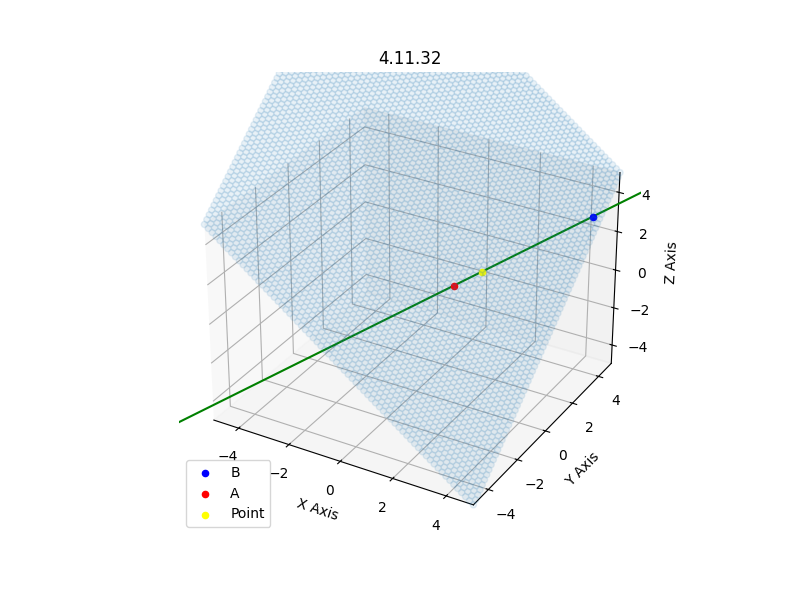
\includegraphics[width=0.8\columnwidth]{../figs/plot.png}
    \caption*{}
    \label{fig:plot}
\end{figure}
\end{frame}

\section{C Code}
\begin{frame}[fragile]{C code for generating points on line}
\begin{lstlisting}[language=C]
 void point_gen(const double* P1, const double* P2, double t, double* result_point) {
    result_point[0] = P1[0] + t * (P2[0] - P1[0]);
    result_point[1] = P1[1] + t * (P2[1] - P1[1]);
    result_point[2] = P1[2] + t * (P2[2] - P1[2]);
}
\end{lstlisting}
\end{frame}

\begin{frame}[fragile]{C code for generating points on plane}
\begin{lstlisting}[language=C]
 void generate_plane_points(
    // Output params
    double* x_coords, double* y_coords, double* z_coords,
    // Grid params
    double x_min, double x_max, int x_steps,
    double y_min, double y_max, int y_steps,
    // Plane stuff
    double n1, double n2, double n3, double c) {
    double x_step_val = (x_max - x_min) / (x_steps - 1);
    double y_step_val = (y_max - y_min) / (y_steps - 1);
    int index = 0;
    for (int i = 0; i < x_steps; i++) {
        for (int j = 0; j < y_steps; j++) {
            double current_x = x_min + i * x_step_val;
            double current_y = y_min + j * y_step_val;
            double current_z;
\end{lstlisting}
\end{frame}
\begin{frame}[fragile]
 \begin{lstlisting}[language=C]
            // Vertical plane check
            if ((c < 1e-9)&&(c > -1e-9)) {
                current_z = 0.0;
            } else {
                current_z = (-n1 * current_x - n2 * current_y + c) / n3;
            }
            x_coords[index] = current_x;
            y_coords[index] = current_y;
            z_coords[index] = current_z;
            index++;
        }
    }
}
 \end{lstlisting}
\end{frame}

\section{Python Code}
\subsection{Using shared objects}
\begin{frame}[fragile]{Python code for plotting using C}
\begin{lstlisting}[language=Python]
import ctypes
import numpy as np
import numpy.linalg as LA
import matplotlib.pyplot as plt
from mpl_toolkits.mplot3d import Axes3D

libline = ctypes.CDLL("./line.so")

get_point = libline.point_gen
get_point.argtypes = [
    ctypes.POINTER(ctypes.c_double),  # P1
    ctypes.POINTER(ctypes.c_double),  # P2
    ctypes.c_double,  # t
    ctypes.POINTER(ctypes.c_double),  # result_point
]
get_point.restype = None
\end{lstlisting}
\end{frame}
\begin{frame}[fragile]
 \begin{lstlisting}[language=Python]
lib = ctypes.CDLL("./plane.so")

lib.generate_plane_points.argtypes = [
    ctypes.POINTER(ctypes.c_double),
    ctypes.POINTER(ctypes.c_double),
    ctypes.POINTER(ctypes.c_double),
    ctypes.c_double,
    ctypes.c_double,
    ctypes.c_int,
    ctypes.c_double,
    ctypes.c_double,
    ctypes.c_int,
    ctypes.c_double,
    ctypes.c_double,
    ctypes.c_double,
    ctypes.c_double,
]
lib.generate_plane_points.restype = None
 \end{lstlisting}
\end{frame}
\begin{frame}[fragile]
 \begin{lstlisting}[language=Python]
DoubleArray3 = ctypes.c_double * 3

a = DoubleArray3(2, -1, 2)
b = DoubleArray3(5, 3, 4)
p = DoubleArray3(2, 0, 3)
q = DoubleArray3(1, 1, 5)
r = DoubleArray3(3, 2, 4)

l1 = DoubleArray3(-28, -41, -18)
l2 = DoubleArray3(32, 39, 22)
n = DoubleArray3(0.2, -0.2, 0.2)
c = 1

fig = plt.figure(figsize=(8, 6))
ax = fig.add_subplot(111, projection="3d")

t_values = np.linspace(0, 1, 100)
line_points_x, line_points_y, line_points_z = [], [], []
 \end{lstlisting}
\end{frame}
\begin{frame}[fragile]
 \begin{lstlisting}[language=Python]
ax.plot(
    line_points_x,
    line_points_y,
    line_points_z,
    color="gray",
)
ax.scatter(b[0], b[1], b[2], color="blue", label="b")
ax.scatter(a[0], a[1], a[2], color="red", label="a")
ax.scatter(c[0], c[1], c[2], color="green", label="Point")

ax.set_xlabel("X Axis")
ax.set_ylabel("Y Axis")
ax.set_zlabel("Z Axis")
ax.set_title("2.9.6")
ax.legend()
ax.grid(True)
plt.savefig("../figs/plot.png")
plt.show()
 \end{lstlisting}
\end{frame}
\subsection{Plot}
\begin{frame}{Plot}
 \begin{figure}[H]
    \centering
    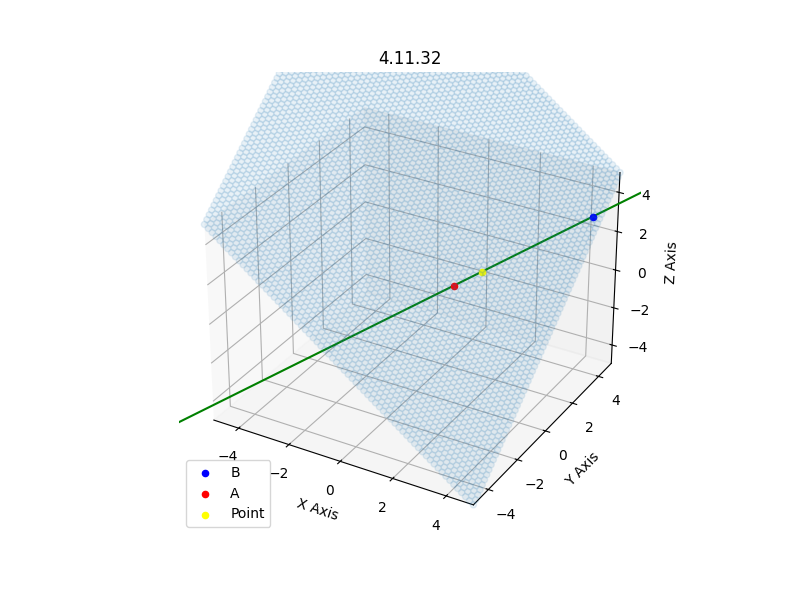
\includegraphics[width=0.8\columnwidth]{../figs/plot.png}
    \caption*{}
    \label{fig:plot}
\end{figure}
\end{frame}
\subsection{In pure Python}
\begin{frame}[fragile]{Pure Python code}
 \begin{lstlisting}[language=Python]
import numpy as np
import matplotlib.pyplot as plt
from mpl_toolkits.mplot3d import Axes3D

a = np.array([5, 1, 6]).T
b = np.array([3, 4, 1]).T
c = np.array([13 / 5, 23 / 5, 0])

fig = plt.figure(figsize=(8, 8))
ax = fig.add_subplot(111, projection="3d")

ax.plot([a[0], c[0]], [a[1], c[1]], [a[2], c[2]], color="blue", label="b")

ax.scatter(b[0], b[1], b[2], color="blue", label="b")
ax.scatter(a[0], a[1], a[2], color="red", label="a")
ax.scatter(c[0], c[1], c[2], color="green", label="Point")
 \end{lstlisting}
\end{frame}
\begin{frame}[fragile]{Pure Python code}
 \begin{lstlisting}[language=Python]
ax.text(a[0], a[1], a[2], "A")
ax.text(b[0], b[1], b[2], "B")
ax.text(c[0], c[1], c[2], "Point")

ax.set_xlabel("X-axis")
ax.set_ylabel("Y-axis")
ax.set_zlabel("Z-axis")
ax.set_title("2.9.6")
ax.set_xlim([-5, 5])
ax.set_ylim([-5, 5])
ax.set_zlim([-5, 5])
ax.legend()
ax.grid(True)

plt.savefig("../figs/python.png")
plt.show()
 \end{lstlisting}
\end{frame}
\subsection{Plot}
\begin{frame}{Plot}
 \begin{figure}[H]
    \centering
    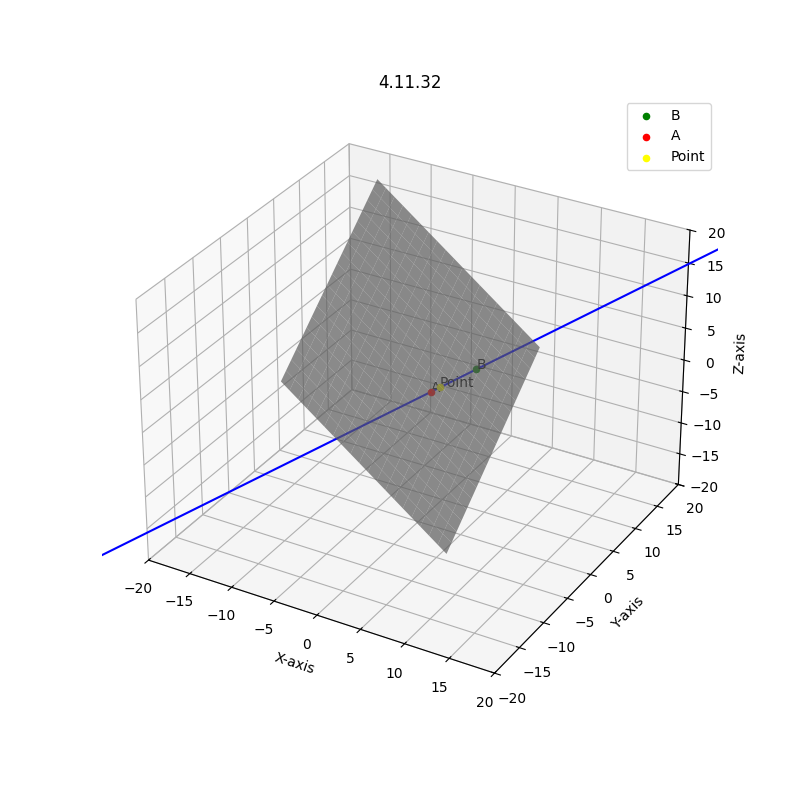
\includegraphics[width=0.75\columnwidth]{../figs/python.png}
    \caption*{}
    \label{fig:plot}
\end{figure}
\end{frame}
\end{document}
